\documentclass{standalone}
\usepackage{pgfplots}
\pgfplotsset{compat=1.18}
\usepackage{xcolor}
\begin{document}
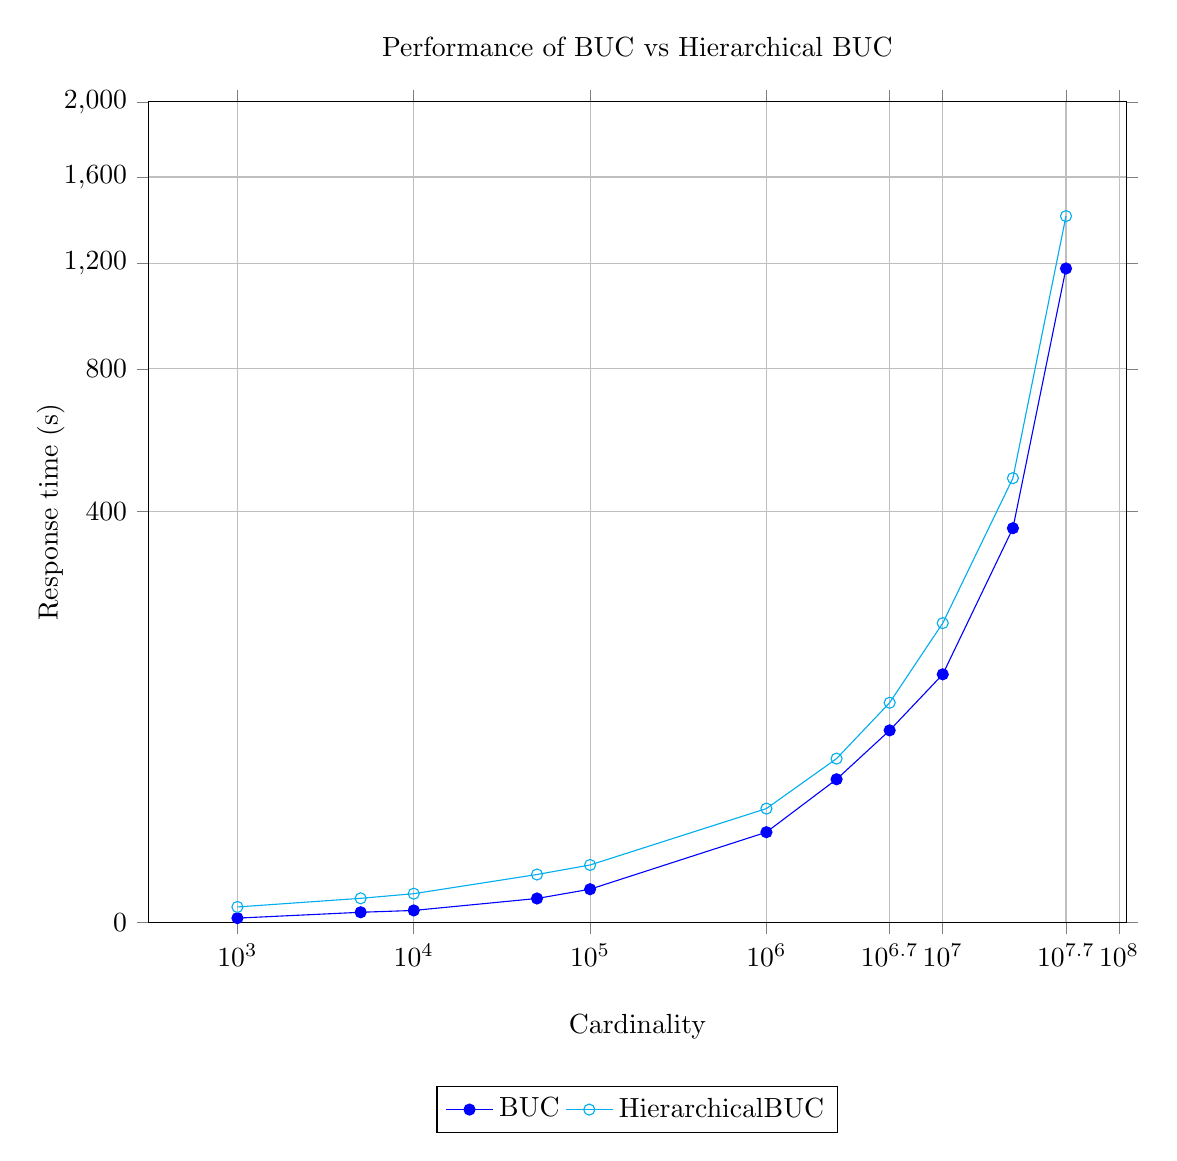
\begin{tikzpicture}
\begin{axis}[
xlabel={Cardinality},
ylabel={Response time (s)},
title={Performance of BUC vs Hierarchical BUC},
title style={yshift=0.7em},
ymode=linear,
y coord trafo/.code={ \pgfmathparse{ (max(#1, 1e-09)/2000)^0.43 } \pgfmathresult },
y coord inv trafo/.code={ \pgfmathparse{ (max(#1, 1e-09)^2.3255813953488373) * 2000 } \pgfmathresult },
ymin=0, ymax=2000,
y label style={at={(axis description cs:-0.1,0.5)},anchor=center},
yticklabel style={/pgf/number format/fixed, /pgf/number format/precision=0},
ytick={ 0,399,800,1199,1599,2000 },
minor y tick num=0,
xmode=log, log basis x=10,
xtick={ 1000,10000,100000,1000000,5000000,10000000,50000000,100000000 },
xmax=110000000.00000001,
xticklabel style={/pgf/number format/sci, /pgf/number format/sci zerofill, /pgf/number format/precision=0},
x label style={at={(axis description cs:0.5,-0.1)},anchor=north},
width=14cm, height=12cm,
grid=major,
legend style={at={(0.5,-0.2)}, anchor=north, legend columns=-1},
tick align=outside,
]
\addplot[color=blue, mark=*] coordinates {(1000,0.0089) (5000,0.06985) (10000,0.1034) (50000,0.52864) (100000,1.13724) (1000000,11.73956) (2500000,34.38212) (5000000,68.12813) (10000000,123.62884) (25000000,363.32039) (50000000,1179.18306)};
\addlegendentry{BUC}
\addplot[color=cyan, mark=o] coordinates {(1000,0.18884) (5000,0.53654) (10000,0.81044) (50000,2.68035) (100000,4.09009) (1000000,20.16265) (2500000,47.05019) (5000000,93.16167) (10000000,191.32115) (25000000,479.64351) (50000000,1410.57157)};
\addlegendentry{HierarchicalBUC}
\end{axis}
\end{tikzpicture}
\end{document}